
\subsection{LTL}
\joerg{OUT. only mention that we can also compile LTL leveraging known
  compilation methods, and exploring this is a topic for future work.}

\rebecca{the compilation of Edelkamp can be used out of the box. If you want to compile multiple properties at 
	the same same time into the planning task (e.g. for the goal dependencies check) you have to use \emph{complete} 
	Büchi automate. Otherwise it is possible that a property influences the result by causing a deadend even if the corresponding
	goal fact it not considered
}

	Example: Package 0 is never in truck 1. $\square ! \text{in}(P_0,T_1)$

	\begin{minipage}{0.22\textwidth}
		\centering
		\tiny
		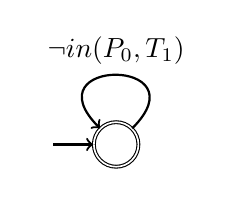
\begin{tikzpicture}
			\node[draw, circle, inner sep=0.2cm, double] (i) at (0,0) {};
			\draw[->, thick, loop] (i) to node[above] {$\neg \text{in}(P_0,T_1)$}(i); 
			\draw[->, thick] (-0.8,0) to (i); 
		\end{tikzpicture}
	\end{minipage}
	\hfill
	\begin{minipage}{0.22\textwidth}
		\centering
		complete \\
		\tiny
		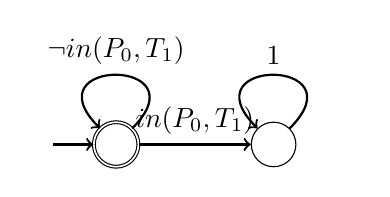
\begin{tikzpicture}
			\node[draw, circle, inner sep=0.2cm, double] (i) at (0,0) {};
			\node[draw, circle, inner sep=0.2cm] (d) at (2,0) {};
			\draw[->, thick, loop] (i) to node[above] {$\neg \text{in}(P_0,T_1)$} (i); 
			\draw[->, thick] (i) to node[above] {$\text{in}(P_0,T_1)$} (d);
			\draw[->, thick, loop] (d) to node[above] {$1$} (d); 
			\draw[->, thick] (-0.8,0) to (i); 
		\end{tikzpicture}
	\end{minipage}

\rebecca{the left automate creates a deadend in the compilation if $P_0$ is not in $T_1$ while the right does not.} 
